\documentclass{standalone}
\usepackage{pgfplots}
\pgfplotsset{compat=newest}
\usetikzlibrary{patterns}
\begin{document}
% \usetikzlibrary{patterns}
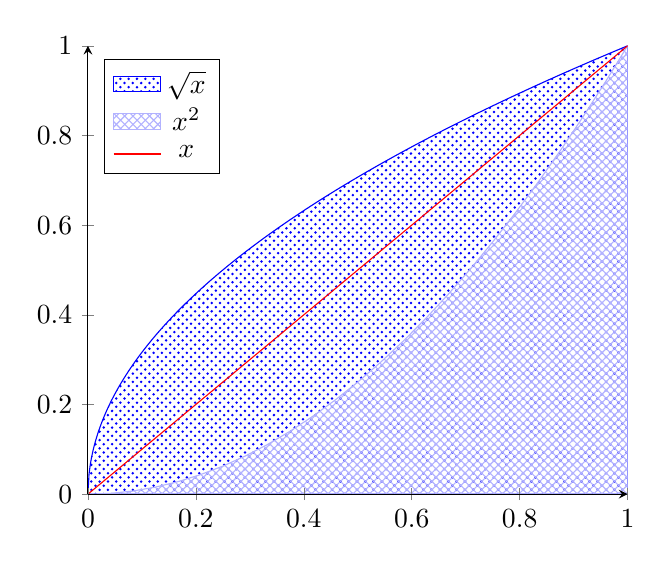
\begin{tikzpicture}
\begin{axis}[area legend,
	axis x line=bottom,
	axis y line=left,
	domain=0:1,
	legend style={at={(0.03,0.97)},
		anchor=north west},
	axis on top,xmin=0]
\addplot[pattern=crosshatch dots,
	pattern color=blue,draw=blue,
	samples=500] 
	{sqrt(x)}	\closedcycle;
\addplot[pattern=crosshatch,
	pattern color=blue!30!white,
	draw=blue!30!white]
	{x^2} \closedcycle;
\addplot[red,line legend] coordinates {(0,0) (1,1)};
\legend{$\sqrt x$,$x^2$,$x$}
\end{axis}
\end{tikzpicture}
\end{document}
